%% ------------------------------------------------------------------------- %%
\chapter{Fundamentação teórica}
\label{cap:fundamentacao-teorica}

De acordo com \cite{Chen-bi-variational-autoencoder:2018}, o objetivo da recuperação de trecho de código-fonte é:

\emph{Recuperar um trecho de código-fonte relevante para atender a necessidade do usuário, descrita em linguagem natural.}

Diversos trabalhos foram feitos com o intuito de sugerir uma forma de recuperar os trechos de código-fonte. Os primeiros trabalhos utilizavam ferramentas baseadas em regras lógico-dedutivas e extração manual de características. As ferramentas baseadas em regras lógico-dedutivas, e.g., o modelo booleano, recuperam informações com base na correspondência exata entre as palavras-chaves e os termos presentes nos trechos de código-fonte. Segundo \cite{yan-benchmark-code-search-information-retrieval-deep-learning:2020}, a correspondência exata dos termos é útil para encontrar informações relativas a erros ou chamadas de \textit{API}, porém é incapaz de recuperar informações relativas a reuso de código ou exemplos de uma biblioteca de programação, onde não há uma correspondência exata entre as palavras-chaves. Nesse caso, há a necessidade de inferir a semântica para conseguir recuperar o trecho de código-fonte.

As redes neurais artificiais surgiram como uma alternativa aos métodos tradicionais de recuperação de informação, pois mostraram-se capazes de inferir a semântica das palavras ou o contexto de frases na busca por documentos ou respostas automáticas a perguntas \citep{guo-deep-look-into-neural-ranking-models:2019}. Atualmente, a maior parte dos trabalhos sobre recuperação de trecho de código-fonte exploram a aprendizagem de máquina utilizando redes neurais artificiais. Tanto que \cite{cambronero-deep-learning-code-search:2019} cunharam o termo \textit{neural code search}, i.e., busca de código-fonte através de redes neurais artificiais. 

A abordagem comumente utilizada busca correlacionar os trechos de códigos-fontes relevantes às intenções de busca do usuário por meio da técnica de agrupamento de vetores contínuos ou \textit{joint embedding}. Essa técnica permite agrupar dados heterogêneos de forma que conceitos semanticamente similares ocupem regiões próximas em um mesmo espaço vetorial \citep{devise-deep-visual-semantic-embedding-frome-2013}. A ilustração dessa técnica pode ser visualizada na Figura~\ref{fig:joint-embedding}.

\begin{figure}[H]
\centering
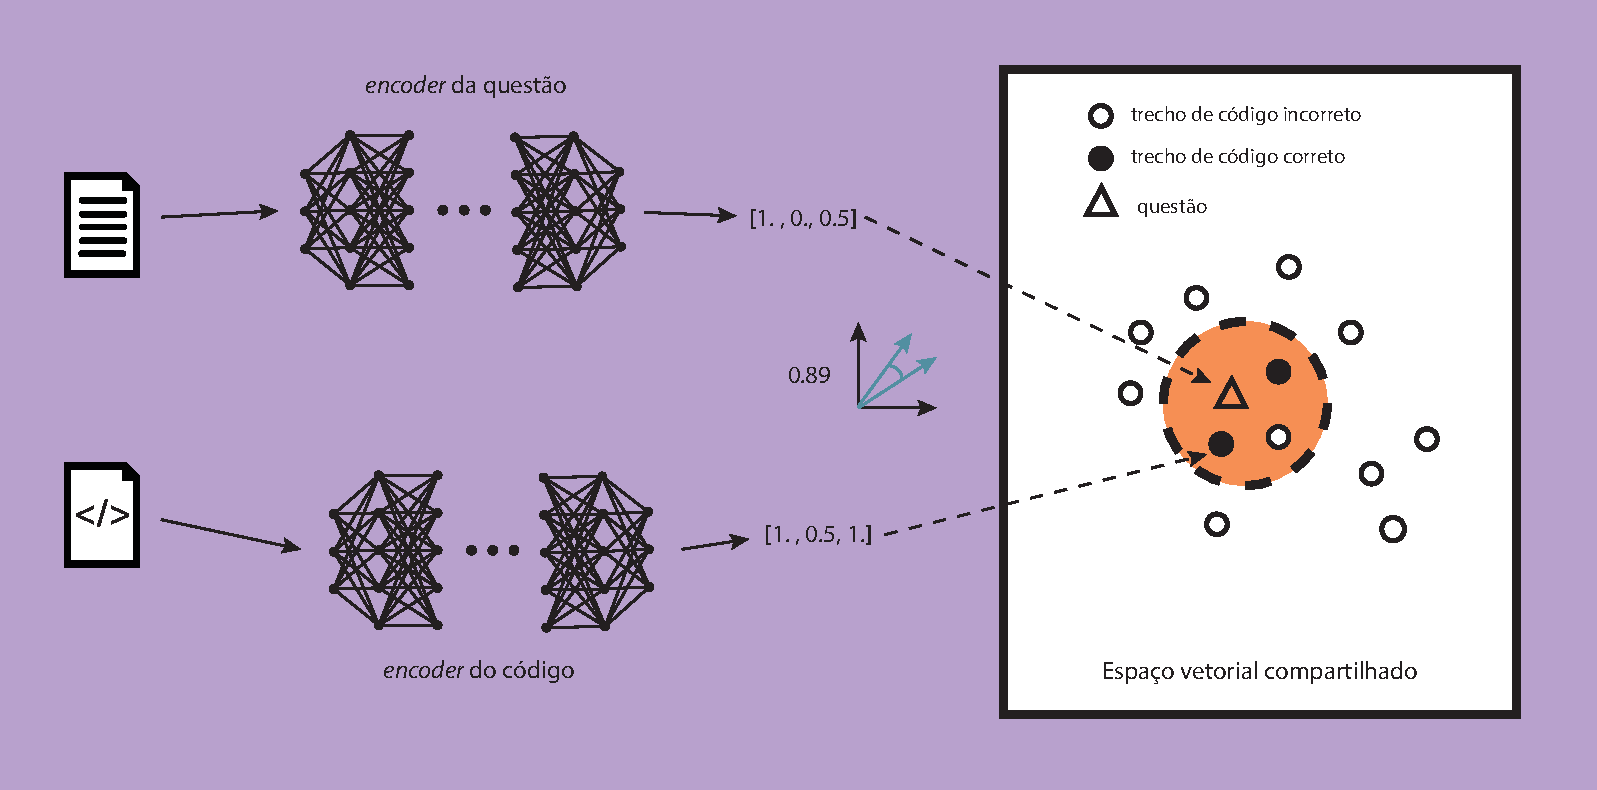
\includegraphics[width=1\textwidth]{figuras/cap-trabalhos-relacionados/joint_embedding.pdf}
\caption{Ilustração da técnica \textit{joint embedding} baseada na figura de \cite{cambronero-deep-learning-code-search:2019}. Duas redes neurais mapeiam os dados de entrada para vetores contínuos. Esses vetores contínuos são agrupados em um mesmo espaço vetorial, de modo que os vetores das questões fiquem próximos aos vetores dos trechos de código-fonte anotados como corretos. A distância entre os vetores pode ser calculada através de uma função de similaridade, e.g., função cosseno ou \textit{cosine}. A rede neural funciona como um codificador ou \textit{encoder} na técnica \textit{joint embedding}, pois a rede neural mapeia os dados de entrada para um vetor contínuo ou \emph{vetor de representação distribuída} em um espaço vetorial de menor dimensão.} 
\label{fig:joint-embedding}
\end{figure}

 No nosso trabalho, as intenções foram expressas através de questões coletadas do \Gls{sof}. Na Figura~\ref{fig:joint-embedding}, ilustramos a técnica \textit{joint embedding} para a recuperação de trecho de código-fonte. Duas redes neurais mapeiam as questões e trechos de código-fonte para vetores contínuos em um mesmo espaço vetorial. Para utilizar essa técnica, três itens devem ser levados em consideração:

\begin{itemize}
    \item Representação dos \textit{tokens} ou palavras
    \item Representação das sentenças
    \item Agrupamento dos vetores contínuos 
\end{itemize}


No primeiro item é necessário definir como os \textit{tokens} ou palavras, que compõem as questões e os trechos de códigos-fontes, serão representadas. No segundo item, os vetores de representação de cada \textit{token} ou palavra serão combinados para obter um vetor contínuo final, que é o vetor de representação da questão ou trecho de código-fonte. Por último, é preciso indicar a função objetivo à rede neural,  preciso indicar à rede neural como agrupar os vetores de representação final das questões e trechos de código-fonte.


\section{\textit{Representação dos \textit{tokens} ou palavras}}
\label{sec:fundamentao-representacao-tokens-palavras}

As questões e os trechos de códigos-fontes são compostas por um conjunto de palavras ou \textit{tokens}. Cada palavra ou \textit{token} deverá ser representado por um vetor numérico. A forma como cada palavra será representada é de extrema importância, pois uma boa representação da palavra auxiliará as redes neurais a correlacionarem as questões aos trechos de código-fonte mais facilmente. Na Figura~\ref{fig:discrete-vs-distributed-representation} ilustramos duas representações típicas para as palavras: vetor de representação esparsa e um vetor de representação distribuída.


\begin{figure}[H]
\centering
\begin{subfigure}{.7\textwidth}
  \centering
  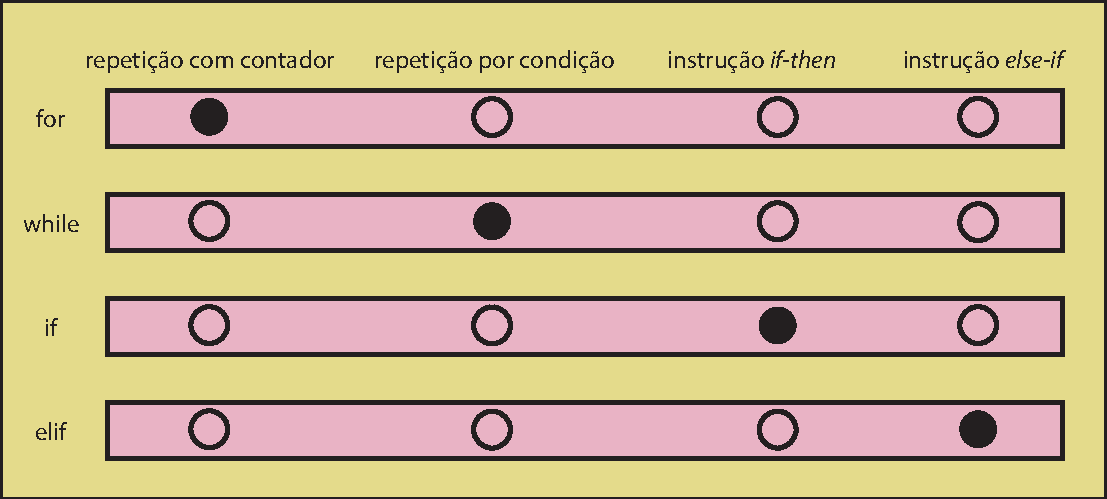
\includegraphics[width=1\linewidth]{figuras/cap-trabalhos-relacionados/discrete-representation.pdf}
  \caption{Ilustração de um vetor de representação esparsa, onde poucos coeficientes são diferentes de zero. Nesse exemplo, cada palavra é representada apenas por um conceito e cada conceito está associado a apenas uma palavra. Uma limitação desse tipo de representação é que o tamanho do vetor cresce de acordo com o tamanho do vocabulário.}
  \label{fig:discrete-representation}
\end{subfigure}%
\\
\begin{subfigure}{.7\textwidth}
  \centering
  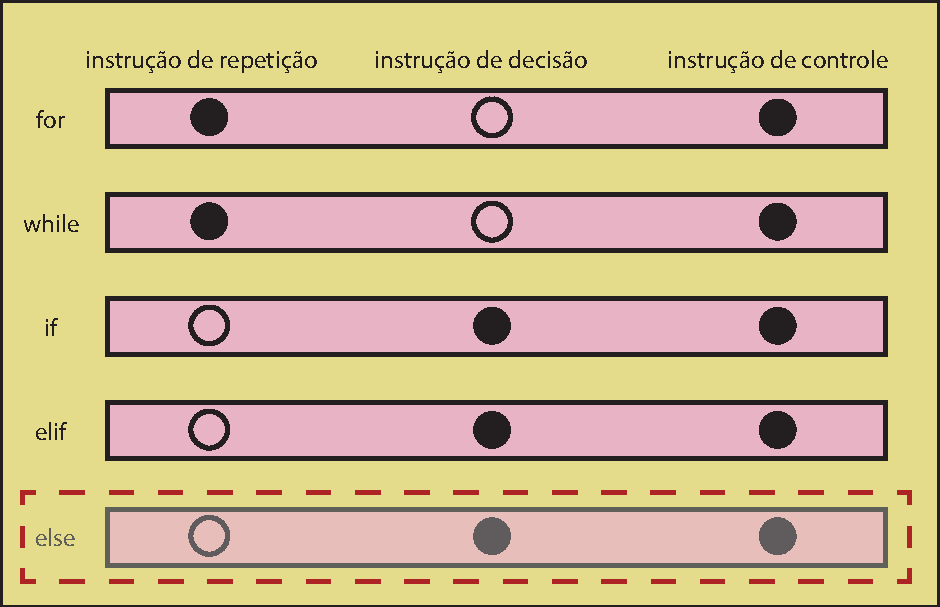
\includegraphics[width=1\linewidth]{figuras/cap-trabalhos-relacionados/distributed-representation.pdf}
  \caption{Ilustração do vetor de representação distribuída, onde cada palavra é representada por vários conceitos e cada conceito está associado a várias palavras \citep{Hinton-distributed-representatons:1986}. No vetor de representação distribuída, o acréscimo de uma nova palavra não aumenta o tamanho do vetor, conforme exibido na Figura.}
  \label{fig:distributed-representation}
\end{subfigure}

\caption{Ilustração de vetores de representação esparsa e distribuída. Ilustração adaptada de: \url{https://www.oreilly.com/content/how-neural-networks-learn-distributed-representations/}}
\label{fig:discrete-vs-distributed-representation}
\end{figure}

O vetor de representação esparsa, conforme a Figura~\ref{fig:discrete-representation}, é composto por poucos coeficientes diferentes de zero. Esse tipo de representação tem duas limitações: o tamanho do vetor cresce de acordo com o tamanho do vocabulário e os coeficientes do vetor não indicam nenhum tipo de relação semântica ou sintática entre as palavras. Já o vetor de representação distribuída é um vetor denso, cujo tamanho é menor que o tamanho do vocabulário de palavras, e o acréscimo de uma palavra não altera a dimensão do vetor. A principal característica dos vetores de representação distribuída é a abstração da relação semântica e/ou sintática através dos seus coeficientes. A Figura~\ref{fig:distributed-representation} ilustra essa característica, onde um coeficiente ou conceito está relacionado a várias palavras e uma palavra está relacionada a vários conceitos, permitindo verificar uma relação entre as palavras através do cálculo de similaridade dos seus respectivos vetores.

 O vetor de representação distribuída utiliza a hipótese distribucional, no qual palavras que estão próximas umas das outras, em diferentes sentenças, tem significados similares \citep{Goodfellow-et-al-2016}. O vetor de representação distribuída de uma palavra é representado por um vetor contínuo ou também chamado de \textit{embedding}. Uma função que mapeia um palavra para um vetor contínuo é chamado de \textit{encoder} ou codificador. Podemos definir \textit{encoder} através da seguinte função \citep{cambronero-deep-learning-code-search:2019}:

\begin{equation}
    f: \mathbb{V} \rightarrow \mathbb{E}
\end{equation}

A função ou \textit{encoder} $f$ mapeia uma palavra $w$, $w \in \mathbb{V}$, para um vetor contínuo $e, e \in \mathbb{E}, \mathbb{E }\subseteq \mathbb{R}^{d}$, onde $\mathbb{V}$ representa o vocabulário de palavras, $\mathbb{E}$ é um conjunto de vetores contínuos e $d$ é a dimensão do vetor. Uma opção comumente utilizada para a função $f$ é o algoritmo não-supervisionado \textit{word2vec}. O \textit{word2vec} recebe uma matriz de inteiros como entrada, onde cada índice da matriz indica uma palavra, e retorna, ao final, uma matriz de vetores contínuos. O \textit{word2vec} tem duas abordagens para obter a matriz de vetores contínuos:

\begin{itemize}
    \item \acrfull{cbow}
    \item \textit{Skip-gram}
\end{itemize}
 
 O \acrshort{cbow} é uma rede neural sequencial que mapeia uma matriz de inteiros para uma matriz de vetores contínuos. Conforme a Figura~\ref{fig:word2vec-cbow}, o \acrshort{cbow} aprende os coeficientes da matriz predizendo uma palavra-alvo a partir de um contexto de palavras ao redor. Já o \textit{Skip-gram} ajusta os coeficientes da matriz predizendo as palavras do contexto a partir de uma palavra central, conforme a Figura~\ref{fig:word2vec-skip-gram}. Essa diferença no método de aprendizagem resulta em vetores contínuos com diferentes características extraídas das palavras. De acordo com \cite{mikolov2013distributed}, o \acrshort{cbow} apresentou bons resultados para tarefas associadas a relações sintáticas das palavras, e.g., associar o adjetivo a advérbio, encontrar o antôninmo ou o superlativo de uma palavra. Enquanto o \textit{Skip-gram} apresentou melhores resultados para associações semânticas como relacionar a cidade a um estado, encontrar a moeda de um país ou associar palavras masculinas e femininas.

\begin{figure}[H]
\centering
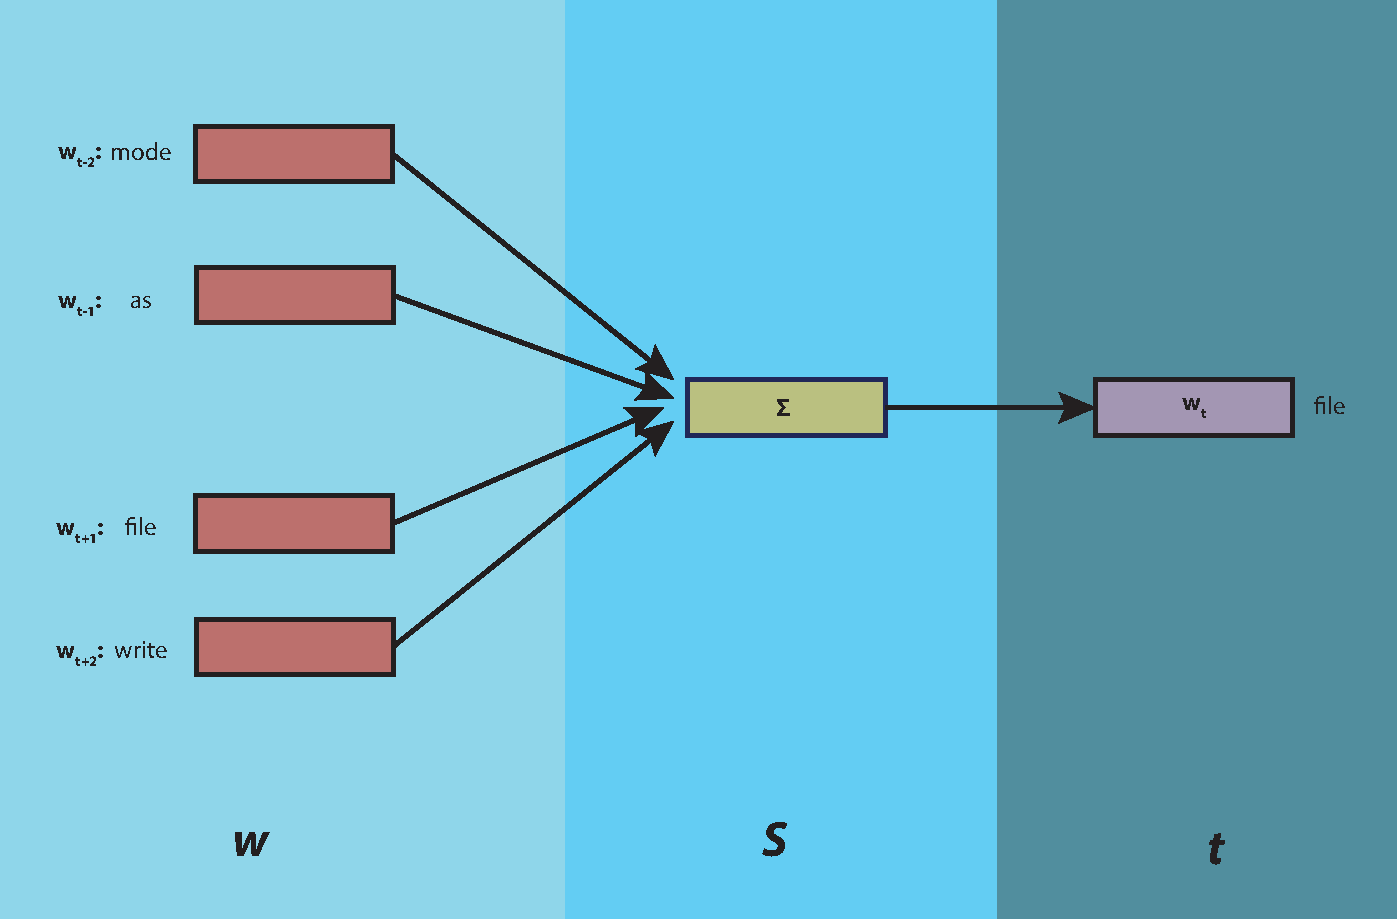
\includegraphics[width=.8\textwidth]{figuras/cap-trabalhos-relacionados/word2vec-cbow.pdf}
\caption{Ilustração da técnica \acrfull{cbow} do \textit{word2vec}. Conforme exibido na Figura, \textit{continuous bag-of-words} prediz uma palavra-alvo $w_{t}$ a partir das palavras do contexto ao redor, $w_{t - 2}, w_{t - 1}, w_{t + 1}, w_{t + 2}$. Imagem baseada na Figura do artigo de \cite{mikolov2013distributed}.} 
\label{fig:word2vec-cbow}
\end{figure}

\begin{figure}[H]
\centering
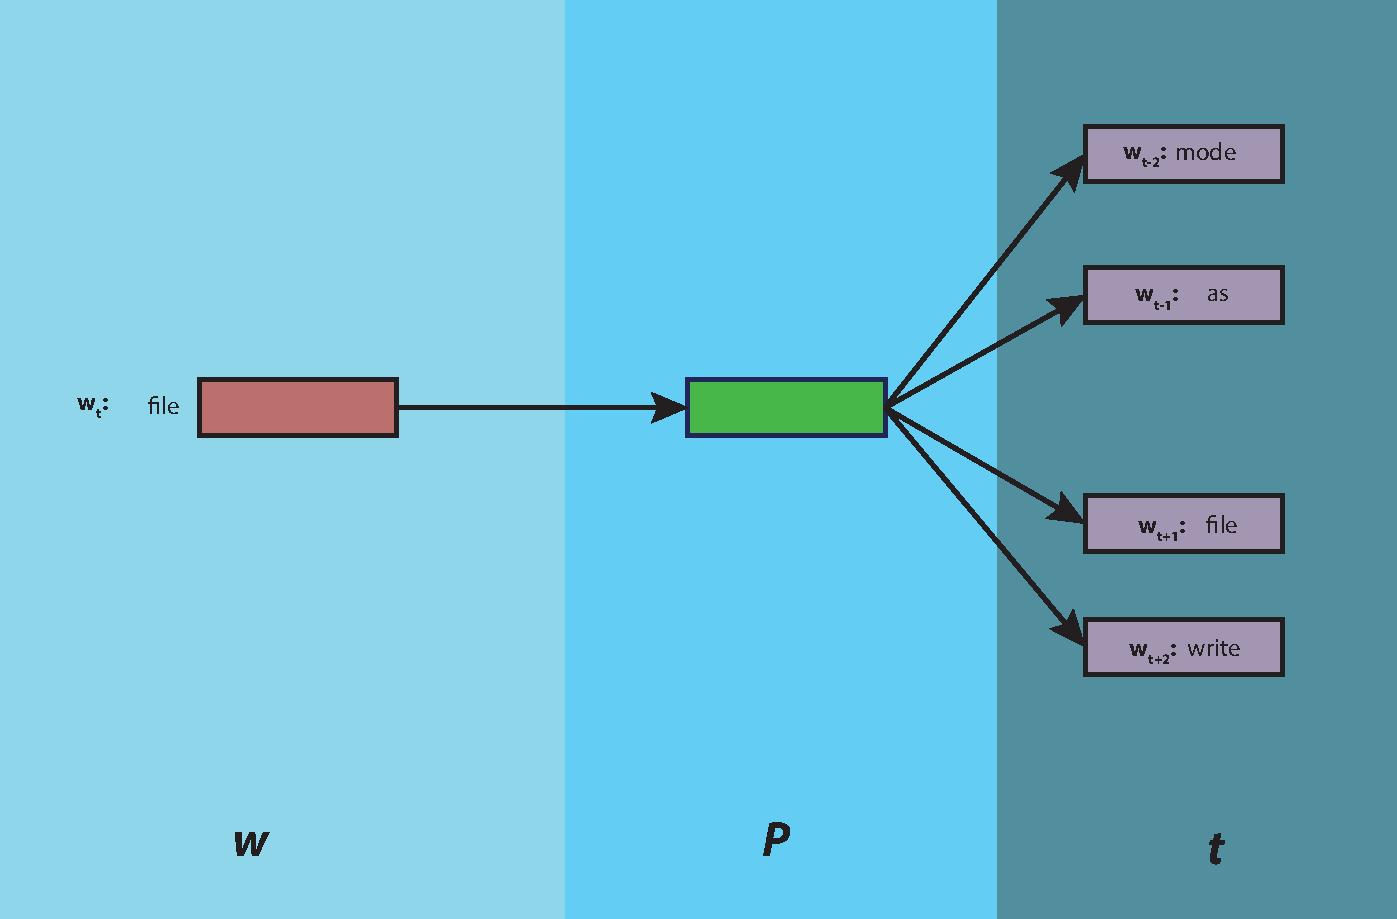
\includegraphics[width=.8\textwidth]{figuras/cap-trabalhos-relacionados/word2vec-skip-gram.pdf}
\caption{Ilustração da técnica \textit{skip-gram} do word2vec. A técnica \textit{skip-gram} prediz as palavras do contexto, $w_{t - 2}, w_{t - 1}, w_{t + 1}, w_{t + 2}$, a partir de uma palavra central $w_{t}$. Ilustração baseada na Figura do artigo de \cite{mikolov2013distributed}. } 
\label{fig:word2vec-skip-gram}
\end{figure}

Para exemplificar o uso do \textit{word2vec}, suponha que tenhamos o seguinte trecho de código-fonte:

\begin{mypython}{Python: Exemplo de código para escrever em um arquivo}
with open(filename, mode) as file:
    file.write(text)
\end{mypython}

Removendo os acentos, tabulações, quebra de linha e as pontuações, o código-fonte pode ser representado por um vetor formado pela seguinte sequência de palavras:

\begin{mypythonembedding}{Trecho de código-fonte representado através de vetor de \textit{tokens}.}
  ['with', 'open', 'filename', 'mode', 'as', 'file', 'file', 'write', 'text']
\end{mypythonembedding}

Nesse caso, ao utilizar o \textit{skip-gram} para a palavra \emph{file} e um parâmetro \textit{window} de valor 2, onde o parâmetro \textit{window} define a quantidade de palavras anteriores e posteriores à palavra central, o algoritmo deverá irá associar a palavra \textit{file} às palavras \emph{mode}, \emph{as}, \emph{file}, \emph{write}.

\begin{mypythonembedding}{Palavra central \textit{file}, em amarelo, e as palavras anteriores e posteriores, em verde, para o parâmetro \textit{window} 2.}
  ['with', 'open', 'filename', |\colorbox{green}{mode}|, |\colorbox{green}{as}|, |\colorbox{yellow}{file}|, |\colorbox{green}{file}|, |\colorbox{green}{write}|, 'text']
\end{mypythonembedding}

O algoritmo \textit{skip-gram} mapeia as palavras que estão perto umas das outras em diferentes contextos para regiões próximas no espaço vetorial $\mathbb{R}^{d}$. No caso da aplicação do \textit{word2vec} em trechos de código-fonte em Python, é possível verificar que a instrução de decisão \emph{if} tem como palavras similares as instruções \emph{elif} e \emph{else}. Já a instrução de repetição \emph{while} tem como instruções similares \emph{continue} e \textit{break}. Enquanto no exemplo anterior, as palavras \emph{file}, \emph{mode}, \emph{as}, \emph{write} serão consideradas similares. 


\section{\textit{Representação das sentenças}}
\label{sec:representacao-das-sentencas-fundamentacao-teorica}

O vetor contínuo de cada palavra pode ser combinado para gerar um vetor para a sentença inteira, e.g., podemos ter um vetor para o trecho de código-fonte, combinando os vetores de cada termo presente no trecho de código. Duas abordagens comumente utilizadas para agrupar os vetores são \citep{cambronero-deep-learning-code-search:2019}:

\begin{itemize}
    \item \textit{Bag-of-words}
    \item Sequencial
\end{itemize}

A diferença básica entre as duas abordagens é a importância relativa dada a ordem das palavras na sentença. No caso do \textit{bag-of-words}, o agrupamento dos vetores não leva a ordem das palavras em consideração, enquanto na abordagem sequencial, os vetores são combinados sequencialmente. O \textit{bag-of-words} normalmente é utilizado em classificação ou recomendação de documentos, onde a frequência de determinadas palavras são mais importantes, enquanto a abordagem sequencial é utilizada em traduções ou análise de sentimentos, pois a ordem das palavras intefere no resultado final. Na Figura~\ref{fig:sentence-representation}, ilustramos as duas abordagens.

\begin{figure}[H]
\centering
\begin{subfigure}{.7\textwidth}
  \centering
  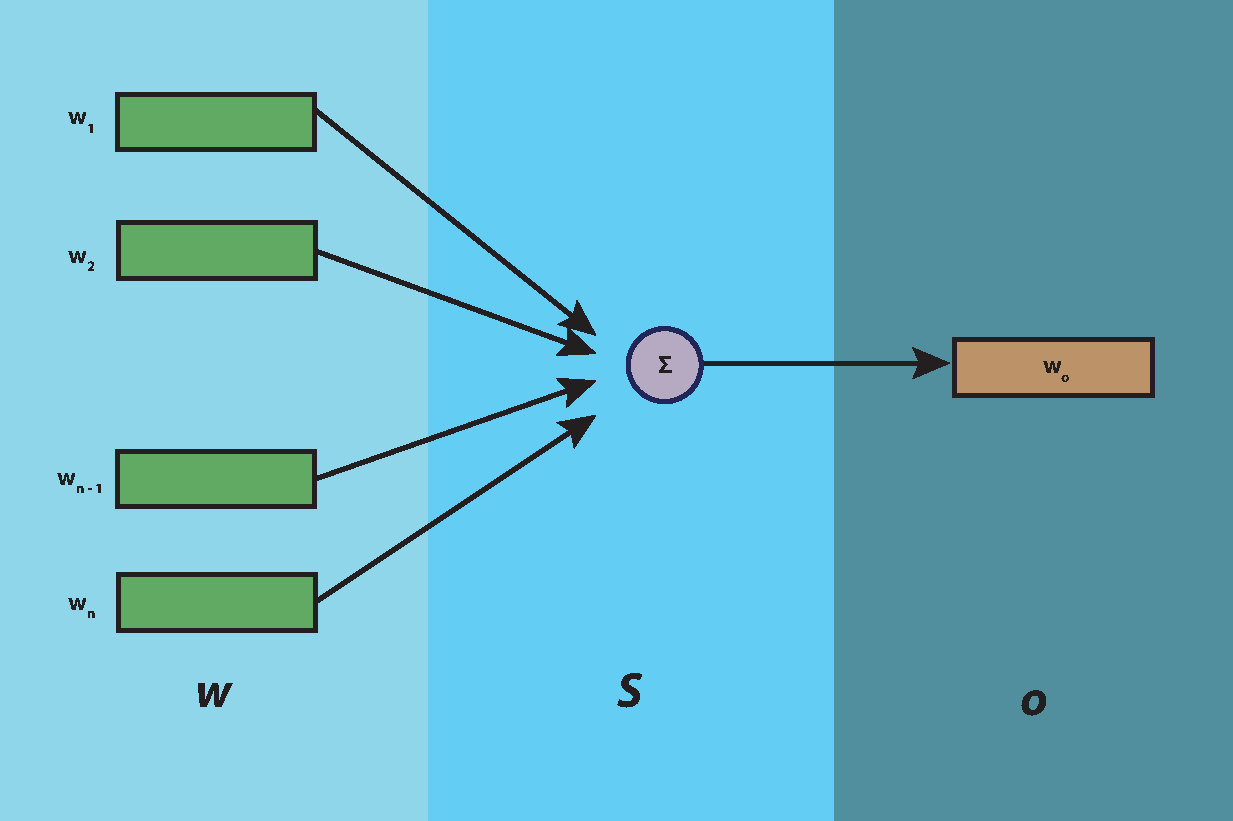
\includegraphics[width=1\linewidth]{figuras/cap-trabalhos-relacionados/sentence-representation-bag-of-words.pdf}
  \caption{Ilustração da abordagem \textit{bag-of-words}. Nesse exemplo, os vetores contínuos de cada palavra são combinados através de uma operação de soma. Ao final, temos um vetor $w_{o}$ que representa a sentença.}
  \label{fig:sentence-representation-bag-of-words}
\end{subfigure}%
\\
\begin{subfigure}{.7\textwidth}
  \centering
  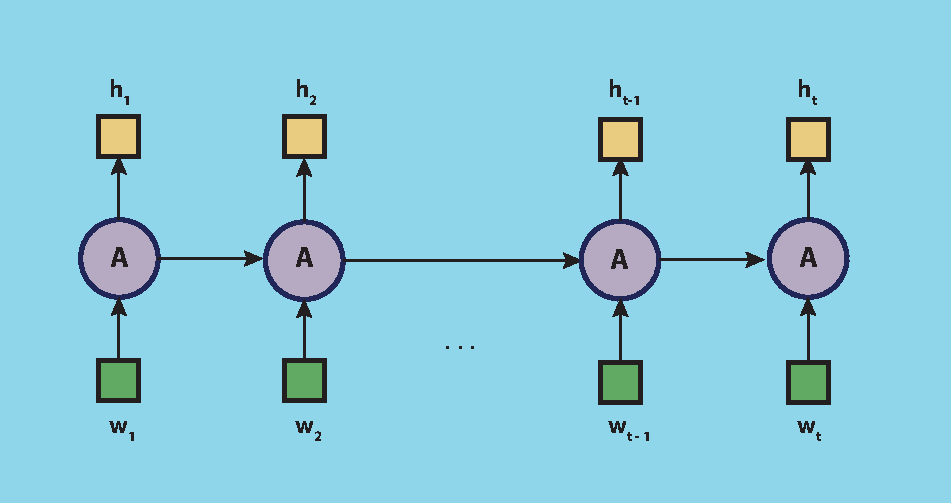
\includegraphics[width=1\linewidth]{figuras/cap-trabalhos-relacionados/sentence-representation-sequential.pdf}
  \caption{Ilustração da abordagem sequencial, onde os vetores são fornecidos individualmente à rede neural. A cada passo $i$, a rede neural \emph{A} combina um vetor da palavra $w_{i}$ com o vetor do resultado anterior $h_{i - 1}$. Ao final de $t$ passos, obtemos o vetor de representação da sentença $h_{t}$. Imagem baseada na figura do website: \url{https://colah.github.io/posts/2015-08-Understanding-LSTMs/}}
  \label{fig:sentence-representation-sequential}
\end{subfigure}

\caption{Ilustração das abordagens \textit{bag-of-words} e sequencial para combinar vetores contínuos de palavras.}
\label{fig:sentence-representation}
\end{figure}


O exemplo de \textit{bag-of-words} ilustrado na Figura~\ref{fig:sentence-representation-bag-of-words} utiliza a função soma para combinar os vetores contínuos das palavras, porém, é possível utilizar outras funções como média ou \emph{max}, por exemplo. Já a abordagem sequencial combina os vetores individualmente, onde a cada passo o vetor é fornecido a uma função ou rede neural e pode ser combinado com o resultado da etapa anterior. De acordo com o exemplo da Figura~\ref{fig:sentence-representation-sequential}, ao final de $t$ passos, obtemos um vetor $h_{t}$, que pode ser utilizado para representar tanto uma questão quanto um trecho de código-fonte. Uma outra maneira de representar uma questão ou trecho de código-fonte seria combinar os $t$ vetores de resultados ($h_{1}, h_{2}, ..., h_{t-1}, h_{t}$) através da função soma ou média, por exemplo. 

Uma boa combinação dos vetores contínuos permite sintetizar as principais características da sentença em um vetor. Para a recuperação de trechos de código-fonte é importante ser possível estabelecer relações semânticas também, onde trechos de código semanticamente similares sejam representadas por vetores similares. Pois, através dessa relação semântica entre os vetores, é possível ensinar a rede neural a correlacionar as questões aos trechos de código-fonte mais facilmente. Além disso, os vetores contínuos das questões e trechos de código-fonte podem ser reutilizados em outras tarefas como recomendação ou sumarização de código-fonte e identificação de linguagem de programação, por exemplo.

\section{Agrupamento dos vetores contínuos}

Os vetores contínuos das questões e trechos de código-fonte podem ser correlacionados através de uma rede neural. Uma abordagem comumente utilizada é o agrupamento de vetores contínuos ou \textit{joint embedding}, que mapeia os vetores das questões e trechos de código-fonte para um mesmo espaço vetorial. O intuito é agrupar os vetores semanticamente, onde conceitos semanticamente similares ocupem regiões próximas no espaço vetorial. Formalmente para um conjunto $\mathbb{Q}$ de questões e $\mathbb{C}$ de trechos de código-fonte, o agrupamento de vetores contínuos pode ser formulado como:

\begin{equation}
        f: q \mapsto t_{q} \mapsto h_{\theta}(t_{q}, t_{c}) \mapsfrom t_{c} \mapsfrom c :g
\end{equation}

A função ou \textit{encoder} $f$ mapeia o vetor $q \in \mathbb{Q}$ para um espaço vetorial $\mathbb{R}^{d}$, onde $d$ é a dimensão. O \textit{encoder} $g$ mapeia o vetor $c \in \mathbb{C}$ para o mesmo espaço vetorial $\mathbb{R}^{d}$. A função $h_{\theta}$ calcula a similaridade entre os vetores $t_{q}$ e $t_{c}$. O objetivo é aproximar as questões aos trechos de código-fonte anotados como solução, i.e., maximizar a função $h_{\theta}$ para um vetor $t_{q}$ e um correspondente vetor $t_{c^{+}}$, anotado como correto. Para realizar a aproximação dos vetores, é necessário definir uma função objetivo à rede neural. De acordo com \cite{guo-deep-look-into-neural-ranking-models:2019}, há três categorias de funções objetivo comumente utilizadas:

\begin{itemize}
    \item Comparação individual ou \textit{pointwise}
    \item Comparação em pares ou \textit{pairwise}
    \item Comparação em lista ou \textit{listwise}
\end{itemize}


\subsection{Comparação individual ou \textit{pointwise}}

Na comparação indidividual ou \textit{pointwise}, a aproximação dos pares de questões e trechos de código-fonte é reduzido a um problema de classificação ou regressão. Para um par $(q_{i}, c_{i})$, o objetivo é maximizar a verossimilhança ou diminuir a diferença entre o resultado da função $h_{\theta}$ e a correspondente classificação $y_{i}$. De uma maneira geral, podemos definir a função objetivo \textit{pointwise} como:

\begin{equation}
    L (h_{\theta}, \mathbb{Y}): \sum_{i} L(y_{i}, h_{\theta}(q_{i}, c_{i})) 
\end{equation}

$\mathbb{Y}$ representa o conjunto das correspondentes classificações anotadas entre os pares de questões e trechos de código-fonte. Para a função $L$, podemos utilizar a função de entropia cruzada ou \textit{cross entropy}, por exemplo:

\begin{equation}
    L (h_{\theta}, \mathbb{Y}): \sum_{i} y_{i} log( h_{\theta}(q_{i}, c_{i})) + (1 - y_{i})log(1 - h_{\theta}(q_{i}, c_{i})) 
\end{equation}

A função $h_{\theta}$ deve estar dentro do intervalo $[0, 1]$ (e.g., função de similaridade cosseno ou \textit{cosine}) e um valor binário pode ser atribuído ao $y_{i}$. De acordo com \cite{guo-deep-look-into-neural-ranking-models:2019, wu-sql-rank-listwise-approach:2018},  \textit{pointwise} apresenta um bom desempenho em classificação e regressão, e.g., indicação da classe de um trecho de código (e.g. correto ou incorreto) ou apontamento da relevância do código-fonte para uma determinada questão. Porém, de acordo com os pesquisadores, a comparação individual não leva em consideração a relativa preferência das informações, não apresentando um bom desempenho em tarefas de classificação e ordenação de um conjunto de informações por relevância, por exemplo. Nesses casos, a utilização da comparação em pares ou em lista é o mais indicado.


\subsection{Comparação em pares ou \textit{pairwise}}
\label{sec:secao-comparacao-em-pares-pairwise}

De acordo com \cite{guo-deep-look-into-neural-ranking-models:2019}, a comparação em pares prioriza a relativa preferência dos itens, ao invés da correta classificação das informações. Diferentemente da comparação individual, onde a função objetivo é resultado da soma da função para cada item, na comparação em pares, o resultado é fruto da soma das permutações de cada par de itens. Formalmente, a função de comparação em pares pode ser definida como:

\begin{equation}
    L (h_{\theta}): \sum_{i} \sum_{j \neq i} L( h_{\theta}(q_{i}, c_{i}^{+}) - h_{\theta}(q_{i}, c_{j}^{-})) 
\end{equation}

 Dado um vetor $q_{i}$, o vetor $c_{i}^{+}$ é preferível ao vetor $c_{j}^{-}$. No caso de recuperação de trecho de código-fonte, o vetor $c_{i}^{+}$ pode ser uma possível solução à questão $q_{i}$, enquanto o vetor $c_{j}^{-}$ representa um trecho de código que não é solução. Para a função $L$, podemos utilizar a função de perda de articulação ou \textit{hinge loss}, por exemplo:

\begin{equation}
    L (h_{\theta}): \sum_{i} \sum_{j \neq i} max(0, 1 - h_{\theta}(q_{i}, c_{i}^{+}) + h_{\theta}(q_{i}, c_{j}^{-})) 
\end{equation}

De acordo com \cite{feng-2015, guo-deep-look-into-neural-ranking-models:2019, wu-sql-rank-listwise-approach:2018}, a aprendizagem através da função de comparação em pares apresentou bons resultados nas tarefas de seleção de respostas e recomendação. Porém, de acordo com \cite{wu-sql-rank-listwise-approach:2018}, a comparação entre os pares apresenta o mesmo problema da comparação individual, ambas as funções não priorizam a ordenação das informações. A relativa preferência entre os pares não reflete a relativa preferência de um conjunto de informações. Nesse caso, de acordo com \cite{wu-sql-rank-listwise-approach:2018}, o mais indicado é utilizar a comparação em lista ou \textit{listwise}.


\subsection{Comparação em lista ou \textit{listwise}}

De acordo com \cite{wu-sql-rank-listwise-approach:2018}, a função de comparação em lista ou \textit{listwise} atribui um valor à lista de itens observados, ao invés de realizar a comparação individualmente. Dado um vetor $q_{i}$ e uma lista de candidatos $T_{i}$, a função de perda \textit{listwise} pode ser definida como \citep{guo-deep-look-into-neural-ranking-models:2019}:

\begin{equation}
    L (h_{\theta}, Y, T): \sum_{i} \sum_{j = 1}^{|T_{i}|} L( y_{i,j}, h_{\theta}(q_{i}, c_{j}))
\end{equation}

Onde $c_{j} \in T_{i}$ e a função de perda $L$ é calculada de acordo com os itens ordenados $y_{i,j}$, de modo que $j$ indica a posição do elemento observado na lista para um vetor $q_{i}$. Uma possível abordagem é maximizar a verossimilhança entre a lista de candidatos $T_{i}$ e uma lista de itens anotados $\pi_{i}$. Neste caso, a função $L$ seria calculada da seguinte maneira \citep{guo-deep-look-into-neural-ranking-models:2019}:

\begin{equation}
    L (h_{\theta}, Y, T): \sum_{i} \sum_{j = 1}^{|\pi_{i}|} log P( y_{i,j} | T_{i}, h_{\theta})
\end{equation}

Onde $P(y_{i,j} | T{i}, h_{\theta})$ é a probabilidade de selectionar o j-ésimo elemento na lista ordenada $\pi_{i}$ com a função $h_{\theta}$:

\begin{equation}
    P(y_{i,j} | T_{i}, h_{\theta}): \frac{exp(h_{\theta}(q_{i}, c_{j}))}{\sum_{k = j}^{\pi_{i}} exp(h_{\theta}(q_{i}, c_{k}))}
\end{equation}

A função $L$ busca encontrar a permutação ótima da lista de candidatos $T_{i}$. De acordo com \cite{guo-deep-look-into-neural-ranking-models:2019}, apesar da comparação em lista ser mais efetivo que a comparação em pares, o custo computacional limita a sua aplicação. O método \textit{listwise} torna-se uma opção para as etapas de reclassificação, onde um número limitado de documentos é avaliado. 

\section{Trabalhos relacionados}\label{sec:code-retrieval-trabalhos-relacionados}

A principal abordagem utilizada na recuperação de trecho de código-fonte é a técnica \textit{joint embedding}. Na Tabela~\ref{table:summary-joint-embedding} apontamos as diferentes abordagens utilizadas pelos trabalhos com relação a composição do par descrição e trecho de código, as técnicas para criação dos vetores contínuos das palavras e das sentenças.


\begin{table}[H]
\centering

\begin{tabular}{ l p{3cm} p{3cm} p{3cm} }
 \hline
 \textbf{Trabalho} & \textbf{Composição} & \textbf{Vetor contínuo das palavras} & \textbf{Vetor contínuo das sentenças} \\
 \hline
\citep{Allamanis-bimodal-source-code-natural-language:2015} & \Gls{token} / Árvore sintática & Modelo Probabilístico & Média / Matriz de conteúdo  \\

\citep{iyer-etal-2016-summarizing} & \Gls{token} & \Gls{one-hot-encoding} & \acrshort{lstm} com \gls{mecanismo-atencao}  \\

\citep{Chen-bi-variational-autoencoder:2018} & \Gls{token} & Bi-\acrshort{vae} & Bi-\acrshort{vae}, Média e \acrshort{mlp}  \\

\citep{Gu-deep-code-search:2018} & \Gls{token} / Nome do método, chamada de API e \Gls{token} & bi-\acrshort{lstm} & \Gls{max-pooling} / \Gls{max-pooling} e \acrshort{mlp}   \\

\citep{Sachdev-neural-code-search:2018} & \Gls{token} & \Gls{skip-gram} & Média / \acrshort{tf-idf}   \\

\citep{cambronero-deep-learning-code-search:2019} & \Gls{token} & \Gls{skip-gram} & Média / \Gls{mecanismo-atencao}   \\

\textit{Nosso trabalho} & \Gls{token} & \Gls{skip-gram} & \acrshort{cnn}   \\

 \hline
\end{tabular}
\caption{Sumário dos trabalhos relacionados à recuperação de trecho de código-fonte. A coluna \emph{Composição} refere-se ao par questão e trecho de código-fonte. Diferentes métodos são separados por barra (''/''), exibindo o método para a questão e posteriormente o método para o código-fonte. Adaptação de \cite{yan-benchmark-code-search-information-retrieval-deep-learning:2020}.}
\label{table:summary-joint-embedding}
\end{table}

Conforme a Tabela~\ref{table:summary-joint-embedding}, a maioria dos trabalhos representaram as palavras através de vetores de representação distribuída (e.g. modelo probabilístico, bi-\acrshort{vae}, \gls{skip-gram}), exceto \cite{iyer-etal-2016-summarizing} que optou por utilizar uma representação esparsa, \gls{one-hot-encoding}. Já em relação a combinação das palavras, i.e., representação da sentença, os trabalhos de \cite{Gu-deep-code-search:2018} e \cite{iyer-etal-2016-summarizing} optaram pelo uso de redes neurais recorrentes, levando em consideração a ordem das palavras. Enquanto os trabalhos de \cite{Chen-bi-variational-autoencoder:2018}, \cite{Sachdev-neural-code-search:2018} e \cite{cambronero-deep-learning-code-search:2019} optaram por uma abordagem mais simples e trataram o vetor de tokens como uma sacola ou \textit{bag}, i.e., indiferente à ordem das palavras na sentença.

Conforme a Tabela~\ref{table:summary-joint-embedding}, todos os trabalhos extraíram as palavras e os termos individuais das questões, i.e., os \textit{tokens}, para compor os vetores. No caso do código-fonte, apenas os trabalhos de \cite{Allamanis-bimodal-source-code-natural-language:2015} e \cite{Gu-deep-code-search:2018} optaram por não compor os vetores através de \textit{tokens}. \cite{Allamanis-bimodal-source-code-natural-language:2015} preferiram compor o vetor do código-fonte por comandos e expressões obtidas por meio de um analisador sintático, priorizando a relação hierárquica entre os termos. Já \cite{Gu-deep-code-search:2018} consideraram mais de um aspecto na composição, os pesquisadores utilizaram o nome do método, a invocação da API e os tokens para a construção do vetor.


Com relação a função objetivo, os trabalhos de \cite{iyer-etal-2016-summarizing} e \cite{Chen-bi-variational-autoencoder:2018} otimizaram o modelo para classificar as respostas corretamente. Ambos os trabalhos utilizaram a função de custo log-verossimilhança negativa, cujo objetivo é maximizar a verossimilhança entre a resposta obtida pelo modelo e as respostas observadas. \cite{Allamanis-bimodal-source-code-natural-language:2015} optou pela função de estimativa do contraste de ruído ou \acrfull{nce}, que busca discriminar as respostas observadas entre uma amostra de ruídos \citep{gutmann-nce-noise-contrastive-estimation-2010}. Diferentemente dos outros trabalhos, \cite{Gu-deep-code-search:2018} utilizou a função de perda de articulação ou \textit{hinge loss}, que prioriza a relativa preferência das respostas corretas, ao invés da sua correta classificação. 

Para avaliação do modelo, há uma diferença com relação ao corpus de busca. Corpus de busca entende-se como um conjunto de dados pela qual um modelo utiliza como fonte de busca das informações. \cite{Gu-deep-code-search:2018}, \cite{Sachdev-neural-code-search:2018} e \cite{cambronero-deep-learning-code-search:2019} utilizaram repositórios do Github para encontrar os trechos de código-fonte. Já \cite{iyer-etal-2016-summarizing} e \cite{Chen-bi-variational-autoencoder:2018} avaliaram o modelo em uma amostra contendo a resposta correta e outros 49 distratores, selecionados aleatoriamente da amostra de treinamento. 

\begin{table}[h]
\centering
\begin{tabular}{ p{8em} p{6em} P{6em} P{8em} P{6em} }
\hline
 &  & \textbf{Treinamento} & \multicolumn{2}{c}{\textbf{Avaliação}} \\
\hline
\textbf{Artigo} & \textbf{Linguagem} & \textbf{\# de dados} & \textbf{\# questões anotadas} & \textbf{Corpus de busca}  \\
\hline

\cite{Allamanis-bimodal-source-code-natural-language:2015} & C\# & $24.812$ & N/D & $50$ \\

\cite{Chen-bi-variational-autoencoder:2018} & \multirow{2}{*}{ C\# / SQL} &
\multirow{2}{*}{ $66.015$ / $25671$} & \multirow{2}{*}{ $100$} & \multirow{2}{*}{ $50$} \\

\cite{iyer-etal-2016-summarizing} &  &  &  &  \\

\cite{Gu-deep-code-search:2018} & Java & $16$ milhões & $50$ & $4$ milhões \\

\cite{Sachdev-neural-code-search:2018} & Java (Android) & $787$ mil & $100$ & $5,5$ milhões \\

\cite{cambronero-deep-learning-code-search:2019} & Java / Java (Android) & $16$ milhões / $787$ mil & $50$ / $287$ & $4$ milhões / $5,5$ milhões \\

 \hline
 
\end{tabular}
\caption{Relação da quantidade de dados utilizada para treinamento e avaliação dos modelos. A coluna \textbf{\# questões anotadas} refere-se a quantidade de questões anotadas manualmente para avaliação final do modelo.}
\label{table:summary-training-data}
\end{table}


De acordo com a Tabela~\ref{table:summary-source-data}, a maioria dos trabalhos utilizaram questões coletadas do \acrfull{sof-ab} como fonte de entrada para a avaliação final do modelo. Já em relação ao corpus de busca, \cite{Gu-deep-code-search:2018}, \cite{Sachdev-neural-code-search:2018} e \cite{cambronero-deep-learning-code-search:2019} utilizaram o \acrfull{github-ab} como fonte, enquanto que \cite{Allamanis-bimodal-source-code-natural-language:2015}, \cite{iyer-etal-2016-summarizing} e \cite{Chen-bi-variational-autoencoder:2018} utilizaram trechos de código coletados do Stack Overflow. A composição dos pares de questões e trechos de código-fonte diferiu de acordo com a fonte dos dados de treinamento. Os trabalhos que utilizaram o \acrfull{github-ab}, compuseram os pares com métodos e \gls{docstring}, enquanto os que utilizaram \acrfull{sof-ab}, formaram os pares pelo título da questão e pelo trecho de código-fonte da resposta aceita.

\begin{table}[h]
\centering
\begin{tabular}{ p{8em} p{5em} p{5em} p{5em} p{5em} p{5em} }
\hline
 & \multicolumn{3}{c}{\textbf{Treinamento}} & \multicolumn{2}{c}{\textbf{Avaliação}} \\
\hline
\textbf{Artigo} & \textbf{Fonte} & \textbf{Questões} & \textbf{Código-Fonte} & \textbf{Fonte das questões} & \textbf{Fonte do corpus de busca}\\
\hline

\cite{Allamanis-bimodal-source-code-natural-language:2015} & \acrshort{sof-ab} & Título da postagem & Trecho de código-fonte & \acrshort{sof-ab} & \acrshort{sof-ab}\\

\cite{Chen-bi-variational-autoencoder:2018} & \acrshort{sof-ab} & Título da postagem & Trecho de código-fonte & \acrshort{sof-ab} & \acrshort{sof-ab}\\

\cite{iyer-etal-2016-summarizing} & \acrshort{sof-ab} & Título da postagem & Trecho de código-fonte & \acrshort{sof-ab} & \acrshort{sof-ab}\\

\cite{Gu-deep-code-search:2018} & \acrshort{github-ab} & Docstring & Método & \acrshort{sof-ab} & \acrshort{github-ab}\\

\cite{Sachdev-neural-code-search:2018} & \acrshort{github-ab} & N/D & Método	& \acrshort{sof-ab} & \acrshort{github-ab}\\

\cite{cambronero-deep-learning-code-search:2019} & \acrshort{github-ab} / \acrshort{sof-ab} & Docstring / Título da postagem & Método / Trecho de código-fonte & \acrshort{sof-ab} & \acrshort{github-ab}\\

 \hline
 
\end{tabular}
\caption{Repositórios utilizados para coleta dos dados de treinamento e avaliação dos modelos no problema de \textit{code retrieval}.}
\label{table:summary-source-data}
\end{table}




De acordo com \cite{cambronero-deep-learning-code-search:2019}, os dados utilizados para compor os pares influenciaram no desempenho final do modelo. Em seu trabalho, foram observados um ganho no desempenho das redes neurais quando treinados com os títulos das questões e trechos de código-fonte do \acrfull{sof-ab}, em comparação aos pares formados por \gls{docstring} e métodos extraídos do \acrfull{github-ab}. Outro fator importante para a aprendizagem do modelo é a variabilidade das questões e trechos de código-fonte. \cite{yao-2018} verificaram que um aumento da variabilidade resultou em um ganho de mais de 10\% no desempenho final de um modelo, sem alteração da sua arquitetura e a devida otimização dos hiper-parâmetros.


A proposta do nosso trabalho foi analisar o desempenho das redes convolucionais na tarefa de recuperação de trechos de código-fonte. Para isto, comparamos a eficácia do nosso modelo com outros dois modelos: um modelo de base de comparação e o outro proposto por \cite{cambronero-deep-learning-code-search:2019}, que é o atual estado da arte. Para o treinamento e avaliação, utilizamos os dados coletados por \cite{yao-2018}, devido 
a maior variabilidade das questões e trechos de código-fonte em comparação aos dados utilizados por \cite{Allamanis-bimodal-source-code-natural-language:2015} e \cite{iyer-etal-2016-summarizing}, por exemplo. 